\section{\numb section 8. A closer look at cells and meshes}

This section gives details about cells and meshes.


\paragraph{\numb section 8.\numb parag 1. Building cells and meshes}

As we have already seen in examples in previous sections, cells and meshes are created
by declaring them as {\codett Cell} or {\codett Mesh} objects and by providing specific
options to their constructor, by means of {\codett tag}s. For instance :

\verbatim
   Cell SW ( tag::vertex ); // and the same for vertices SE, NE, NW
   Mesh south ( tag::segment, SW.reverse(), SE, tag::divided_in, 10 );
   // similar declarations of east, north, west
   Mesh rectangle ( tag::rectangle, south, east, north, west );
\endverbatim

Paragraph \numb section 9.\numb parag 2 gives more details about {\codett tag}s.

Internally, {\maniFEM} implements cells and meshes as persistent objects, built
using the {\codett new} operator and thus having no syntactic scope.
Objects belonging to classes {\codett Cell} and {\codett Mesh} are just a wrapper
around a persistent core (cell or mesh).
When they go out of scope, the wrappers are destroyed but the core remains alive.
If a cell or mesh is no longer needed, the user must explicitly dispose of it,
as explained in paragraph \numb section 9.\numb parag 3.

Cells and meshes are unique objects, it makes no sense to copy them.
A statement like {\codett Cell copy\_of\_A = A} will make a copy of the wrapper
but it will refer to the same cell {\codett A}.
If you change e.g.\ a coordinate of {\codett copy\_of\_A}, the coordinate of {\codett A}
will also change.
That is, wrapper classes {\codett Cell} and {\codett Mesh} can be viewed as
customized pointers.
This is useful if we need to create many meshes in a loop, as shown in paragraph
\numb section 8.\numb parag 2.
However, there are operations which do create a new cell or mesh.
There are also operations which create a new cell or mesh only if necessary,
otherwise they will return an existing cell or mesh.
Paragraph \numb section 8.\numb parag 10 gives a complete list.

Recall that, in \maniFEM, cells and meshes are oriented.
When a cell is declared, it is built as positive and has no reverse.
Its reverse is a negative cell and will be built only if necessary.
Cells have a method {\codett reverse} which does the following.
It checks if the reverse object has already been built; if yes, it returns that object;
otherwise, it builds the reverse cell on-the-fly and returns it.
Paragraph \numb section 8.\numb parag 7 gives a more detailed explanation about
orientation of cells and meshes.
% See also paragraph \numb section 9.\numb parag 6.

{\codett Mesh}es have also a {\codett reverse} method.
Note that reverse meshes exist always (negative meshes are temporary objects built
on-the-fly).

At a basic level, the only situation when you need the {\codett reverse} method  for cells is
when you declare a segment {\codett Mesh} (you must provide a negative {\codett Cell} as
starting point).
You will occasionaly need to use the {\codett reverse} method for meshes (for instance, if you
intend to {\codett join} two meshes, their common boundary must have a certain orientation when
seen from a mesh and the opposite orientation when seen from the other mesh).
In the example in paragraph \numb section 1.\numb parag 3,
reverses of meshes {\codett CD} and {\codett BC} are used.


\vfil\eject

\paragraph{\numb section 8.\numb parag 2. A ring-shaped mesh}

For creating many meshes within a cycle, we can view a {\codett Cell} object as a
(customized) pointer to a persistent core cell, and the same for {\codett Mesh}es.
They are cheap to store and to copy.
We call these customized pointers ``wrappers''; their behaviour is described in some detail in
paragraph \numb section 9.\numb parag 3.

\verbatim
   Manifold RR2 ( tag::Euclid, tag::of_dim, 2 );
   Function xy = RR2.build_coordinate_system ( tag::Lagrange, tag::of_degree, 1 );
   Function x = xy[0],  y = xy[1];

   short int n_sectors = 15;
   double step_theta = 8*atan(1.)/n_sectors;
   short int radial_divisions = 10;
   short int rot_divisions = 5;
\endverbatim
   
\centerline{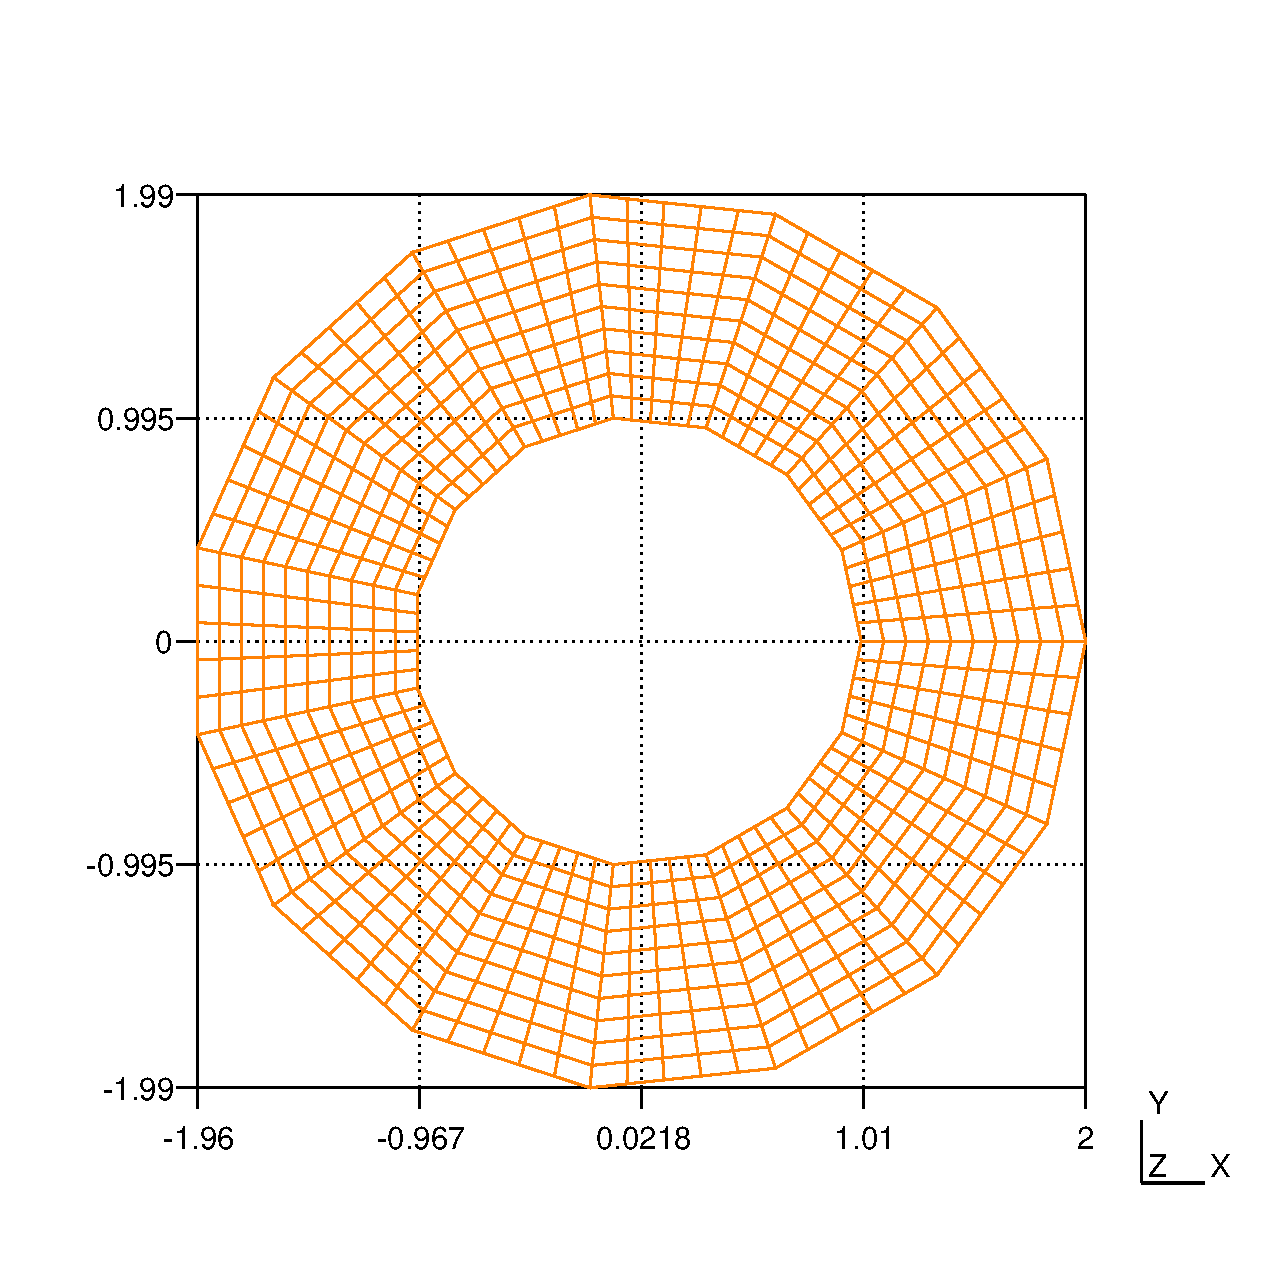
\includegraphics[width=10cm]{ring.eps}}

\verbatim
   // start the process by building a segment
   Cell ini_A ( tag::vertex );  x(ini_A) = 1.;  y(ini_A) = 0.;
   Cell ini_B ( tag::vertex );  x(ini_B) = 2.;  y(ini_B) = 0.;
   Mesh ini_seg ( tag::segment, ini_A.reverse(), ini_B,
                  tag::divided_in, radial_divisions     );
   Mesh prev_seg = ini_seg;
   Cell A = ini_A,  B = ini_B;
   list < Mesh > sectors;

   for ( short int i = 1; i < n_sectors; i++ )
   {  double theta = i * step_theta;
      // we build two new points
      Cell C ( tag::vertex ); x(C) = cos(theta);    y(C) = sin(theta);
      Cell D ( tag::vertex ); x(D) = 2.*cos(theta); y(D) = 2.*sin(theta);
      // and three new segments
      Mesh BD ( tag::segment, B.reverse(), D, tag::divided_in, rot_divisions );
      Mesh DC ( tag::segment, D.reverse(), C, tag::divided_in, radial_divisions );
      Mesh CA ( tag::segment, C.reverse(), A, tag::divided_in, rot_divisions );
      Mesh quadr ( tag::quadrangle, prev_seg, BD, DC, CA );
      sectors.push_back ( quadr );
      prev_seg = DC.reverse();
      A = C;  B = D;                                                     }

   // we now build the last sector, thus closing the ring
   // prev_seg, A and B have rotated during the construction process
   // but ini_seg, ini_A and ini_B are the same, initial, ones
   Mesh outer ( tag::segment, B.reverse(), ini_B, tag::divided_in, rot_divisions );
   Mesh inner ( tag::segment, ini_A.reverse(), A, tag::divided_in, rot_divisions );
   Mesh quadr ( tag::quadrangle, outer, ini_seg.reverse(), inner, prev_seg );
   sectors.push_back ( quadr );
   
   Mesh ring ( tag::join, sectors );
   ring.export_msh ("ring.msh");
\endverbatim

Note how we use a version of the {\codett Mesh} constructor with {\codett tag::join} taking as
argument a list of {\codett Mesh}es; we have already seen it in paragraph \numb section 2.\numb
parag 6.

We might have set curved boundaries by using a submanifold of $ \RR^2 $, like in paragraph
\numb section 2.\numb parag 8.

See also paragraph \numb section 9.\numb parag 7.


\paragraph{\numb section 8.\numb parag 3. Lists of cells inside a mesh}

As explained in paragraph \numb section 1.\numb parag 2, a {\codett Mesh} is
roughly a list of cells.
Internally, {\maniFEM} keeps lists of cells of each dimension, up the the maximum
dimension which is the dimension of the mesh.
Thus, if {\codett msh} is a {\codett Mesh} object, modelling a
mesh of triangles, then {\codett msh.core->cells[0]} is a list of pointers to cells holding
all vertices of that mesh, {\codett msh.core->cells[1]} is a list of pointers to cells
holding all segments and {\codett msh.core-> cells[2]} is a list of pointers to cells
holding all triangles.

Thus, we could use a loop like the one below for iterating over all segments of the mesh.

\verbatim
   for ( auto it = msh.core->cells[1].begin();
              it != msh.core->cells[1].end();  it++ )
   { auto seg = *it;  do_something_to (*seg);  }
\endverbatim

If you are not familiar with the notion of iterator over a list (or over other containers)
in {\tt C++}, this may be a good time for you to read an introductory book on the
{\tt C++} Standard Template Library (STL).

The {\codett auto} keyword tells the {\tt C++} compiler to guess the type of a variable
according to the expression used to initialize it.

Note that the above code only works for a positive mesh.
Paragraphs \numb section 8.\numb parag 5 and \numb section 8.\numb parag 6 describe
nicer ways to iterate over cells of a mesh.

On the other hand, a cell is roughly defined by its boundary which in turn is a mesh of
lower dimension.
Thus, if {\codett hex} is a {\codett Cell} object modelling a hexagon,
then {\codett hex.boundary()} is a {\codett Mesh} object modelling a
one-dimensional mesh (a closed chain of six segments).
So, if we want to iterate, say, over all vertices of that hexagon, we can use a 
loop like below.

\verbatim
   auto & li = hex.boundary().cells[0];
   for ( auto it = li.begin(); it != li.end(); it++ )
   { auto P = *it;  do_something_to (*P);  }
\endverbatim

Note that the above only works if {\codett hex} is a positive cell.
Also, we have no guarantee about the order in which the vertices will show up in the loop.
Paragraph \numb section 8.\numb parag 6 describes other ways of iterating over one-dimensional
meshes, which follow the natural order of the vertices or segments.


\paragraph{\numb section 8.\numb parag 5. Iterators over cells}

This paragraph assumes that the reader is familiar to the notion of iterator in {\tt C++}.
If this is not the case, you should read an introductory book on the {\tt C++}
Standard Template Library (STL) before proceeding.

As explained in paragraphs \numb section 1.\numb parag 2 and \numb section 8.\numb parag 3,
a mesh is essentially a collection of cells.
In many situations, we may want to iterate over all cells of a mesh.

Suppose we have a mesh {\codett msh} of rectangles.
If we want to do something to each rectangle, that is, to each two-dimensional cell,
we could use a code like

\verbatim
   for ( auto it = msh.core->cells[2].begin();
              it != msh.core->cells[2].end(); it++ )
   {  auto cll = *it;  do_something_to (*cll);  }
\endverbatim

This style is slightly cumbersome and doesn't work for negative meshes,
so we provide specific iterators.
The code above is equivalent to

\verbatim
   CellIterator it = msh.iter_over ( tag::cells_of_dim, 2 );
   for ( it.reset(); it.in_range(); it++ )
   {  Cell cll = *it;  do_something_to (cll);  }
\endverbatim

Paragraph \numb section 9.\numb parag 2 gives some details about tags.

In the above code you may note that these iterators obey to syntactic conventions
slightly different from the ones in the Standard Template Library.
We have chosen that, when we want to start an iteration process, we set the iterator in
a starting configuration by using a {\codett reset} method rather than through an assignment
like {\codett it = container.begin()}.
Similarly, when an iterator has offered access to all cells of a mesh and cannot find
other cells, it goes into a state which can be checked using its {\codett in\_range} method
rather than by testing equality with some abstract object like {\codett container.end()}.
We have kept the syntax {\codett it++} for advancing an iterator in the process of
running over cells, offering also the equivalent alteratives {\codett ++it} and
{\codett it.advance()}.
We have also kept the notation {\codett *it} for dereferencing a {\codett CellIterator};
this operation returns a reference to a {\codett Cell} object.
Of course, dereferencing a {\codett CellIterator} does not produce a new cell,
just provides access to a previously built cell (see also paragraph \numb section 8.\numb
parag 10).

If we want to iterate over all vertices of the mesh, we can use

\verbatim
   CellIterator it = msh.iter_over ( tag::cells_of_dim, 0 );
   for ( it.reset(); it.in_range(); it++ )
   {  Cell P = *it;  do_something_to (P);  }
   // or, equivalently :
   CellIterator it = msh.iter_over ( tag::vertices );
\endverbatim

If we want to iterate over all segments of the mesh, we can use

\verbatim
   CellIterator it = msh.iter_over ( tag::cells_of_dim, 1 );
   for ( it.reset(); it.in_range(); it++ )
   {  Cell seg = *it;  do_something_to (seg);  }
   // or, equivalently :
   CellIterator it = msh.iter_over ( tag::segments );
\endverbatim

Note that an iterator running through cells of maximum dimension, that is, of dimension equal
to the dimension of the mesh, may produce negative cells if the mesh contains them.
Paragraph \numb section 8.\numb parag 7 discusses this possibility.
Iterators over cells of lower dimension produce always positive cells.

We can force an iterator over cells of maximum dimension to produce only positive cells
by adding a {\codett tag::force\_positive} as in

\verbatim
   CellIterator it = msh.iter_over ( tag::cells_of_dim, 2, tag::force_positive );
\endverbatim

Note that it is not safe to modify a mesh while iterating over its cells.
After modifying a mesh, you may re-use a previously declared iterator by {\codett reset}ting it.
An exception to the above rule happens for one-dimensional meshes, described in paragraph
\numb section 8.\numb parag 6.

If we only want to know how many cells there are in a certain mesh,
instead of using {\codett msh.core->cells[d].size()} ({\codett d} being the desired
dimension of the cells) we may use the method {\codett number\_of} :

\verbatim
   short int d = 2;
   size_t n = msh.number_of ( tag::cells_of_dim, d );
\endverbatim

\noindent Expression {\codett msh.number\_of ( tag::vertices )} is equivalent to
{\codett msh.number\_of ( tag::cells\_ \_of\_dim, 0 )}, while {\codett msh.number\_of
( tag::segments ) } is equivalent to {\codett msh.number\_of ( tag:: ::cells\_of\_dim, 1 )}.

Paragraph \numb section 8.\numb parag 6 describes iterators specific to one-dimensional
meshes.


\paragraph{\numb section 8.\numb parag 6. Iterators over chains of segments}

One-dimensional meshes have a specific structure (technical details provided in
paragraph \numb section 9.\numb parag 14) so we provide specialized iterators.
Unlike the iterators described in paragraph \numb section 8.\numb parag 5,
which sweep the mesh in a rather unpredictible order,
the iterators below follow the natural order of the cells (either vertices or segments)
given by the topology of the mesh.

The syntax is the same as for higher-dimensional meshes :

\verbatim
   Mesh chain ( tag::segment, A.reverse(), B, tag::divided_in, n );
   // A and B are (positive) vertices, n is an integer
   
   CellIterator it1 = chain.iter_over ( tag::cells_of_dim, 1 );
   for ( it1.reset(); it1.in_range(); it1++ )
   {  Cell seg = *it1;  do_something_to (seg);  }
   
   CellIterator it0 = chain.iter_over ( tag::cells_of_dim, 0 );
   for ( it0.reset(); it0.in_range(); it0++ )
   {  Cell P = *it0;  do_something_to (P);  }

   // or, equivalently,
   CellIterator it0 = chain.iter_over ( tag::vertices );
   CellIterator it1 = chain.iter_over ( tag::segments );
\endverbatim

Unlike iterators over cells of meshes of dimension 2 or higher, presented in paragraph
\numb section 8.\numb parag 5, iterators over one-dimensional meshes require the mesh
to be connected.

A connected one dimensional mesh can be either an open chain of segments or a closed one
(a loop).
For an open chain, {\codett it0} will begin at the first vertex and end at the last vertex,
{\codett it1} will begin at the first segment and end at the last segment.
For a loop, they will begin at some arbitrary vertex or segment in the chain and produce
all the vertices or segments following the natural order given by the topology of the mesh.

If we want to start at a specific location, we can make a {\codett reset} call with
one argument.
For iterators over vertices, this argument should be a vertex, while for iterators
over segments, this argument should be a segment.
If such an argument is given, then the iteration process will begin at that particular
vertex or segment.
This special kind of {\codett reset} can be used for an open chain or a closed one,
but beware : if applied to an open chain, the vertices or segments previous to the provided
argument will not show up in the iteration process.

Note that {\codett it0} produces positive points, while {\codett  it1} produces
oriented segments (positive or negative).
We may enforce that we only want positive segments by adding the {\codett tag::force\_positive},
as shown in paragraph \numb section 8.\numb parag 7.

There are also reversed versions of these iterators (they go backwards), obtained by adding
the {\codett tag::reverse} :

\verbatim
   CellIterator it1r = chain.iter_over ( tag::segments, tag::reverse );
   CellIterator it0r = chain.iter_over ( tag::vertices, tag::reverse );
\endverbatim

Method {\codett number\_of} works just as for higher-dimensional iterators (see paragraph
\numb section 8.\numb parag 5).

One-dimensional meshes have also methods {\codett first\_vertex}, {\codett last\_vertex},
{\codett first\_segment} and {\codett last\_segment} which return the cell described by their
names.
They should only be used for an open chain (not for a loop).
Note that both {\codett Mesh::first\_vertex} and {\codett Mesh::last\_vertex} return
positive vertices, unlike the {\codett Cell::base} method (described in paragraph
\numb section 1.\numb parag 2) which returns a negative vertex. [this should change]

Recall that it is not safe to modify a mesh while iterating over its cells.
After modifying a mesh, you may re-use a previously declared iterator by {\codett reset}ting it.
However, if you modify a one-dimensional mesh and change its topology
(cut a loop, thus making it an open chain, or contrarywise, close a chain,
thus making it a loop), then you cannot re-use
a previously declared iterator on that mesh (you must declare a new iterator).
A change in the code is planned; when we {\codett reset} an iterator, it will adapt itself
to the new shape of the mesh.

As explained in paragraph \numb section 8.\numb parag 10, dereferencing a {\codett CellIterator}
does not produce a new cell, just provides access to a previously built cell.


\paragraph{\numb section 8.\numb parag 7. Orientation of cells inside a mesh}

In \maniFEM, all cells and meshes are oriented.

This can be confusing sometimes, so let's have a closer look at a particular example.

{ \psfrag{A}{\special{ps: gsave 0 0 0.8 setrgbcolor}{\codett A}\special{ps: grestore}}
\psfrag{B}{\special{ps: gsave 0 0 0.8 setrgbcolor}{\codett B}\special{ps: grestore}}
\psfrag{C}{\special{ps: gsave 0 0 0.8 setrgbcolor}{\codett C}\special{ps: grestore}}
\psfrag{D}{\special{ps: gsave 0 0 0.8 setrgbcolor}{\codett D}\special{ps: grestore}}
\centerline{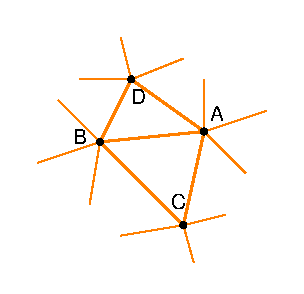
\includegraphics[width=4cm]{malha-tri.eps}} }

Consider a mesh {\codett tri\_mesh} made of triangles.
Unless requested otherwise, {\codett tri\_mesh} will be a positive mesh and all triangles
composing it will also be positive.
So, the triangles composing {\codett tri\_mesh} will have no reverse cell
(there is no need for such).

However, the segments must have reverse.
Consider triangle {\codett ABC} for instance.
Its boundary is made of three segments; let's look at {\codett AB} for example,
a segment having {\codett A} as base and {\codett B} as tip.
Now, a triangle {\codett BAD} (no offense intended) also exists as part of {\codett tri\_mesh}.
The boundary of {\codett BAD} is made of three segments, one of them being {\codett BA},
which has {\codett B} as base and {\codett A} as tip.
{\codett AB} and {\codett BA} are different {\codett Cell} objects;
each is the reverse of the other.
One of them is considered positive and the other is considered negative.
Which is which depends on which one was built first.
So, all inner segments must have a reverse;
segments on the boundary of {\codett tri\_mesh} will probably have no reverse.

For points (vertices), the situation is even more complex.
Segment {\codett AB} sees {\codett A} as negative because {\codett A} is its base,
but other segments like {\codett CA} see {\codett A} as positive.

Let's look again at iterators described in paragraph \numb section 8.\numb parag 5.
We now understand that there is no point to have an iterator over oriented
segments, or over oriented vertices, of {\codett tri\_mesh}.
That's why iterators over cells of lower dimension always produce positive cells.

We also understand that there is no difference between these two iterators :

\verbatim
   CellIterator it1 = tri_msh.iter_over ( tag::cells_of_dim, 2 );
   CellIterator it2 =
      tri_msh.iter_over ( tag::cells_of_dim, 2, tag::force_positive );
\endverbatim

\noindent because all triangles composing {\codett tri\_mesh} should be positive
(use {\codett it1}, it is slightly faster).
However, if some of the triangles are negative {\codett it1} will behave differently from
{\codett it2}.
For instance, if {\codett tri\_mesh} is the boundary of a polyhedron in $ \RR^3 $
and this polyhedron touches other polyhedra (there are shared faces), then it is
quite possible that some of the triangles in {\codett tri\_mesh} be negative.
If you are aware that your mesh may contain negative cells but
you want to iterate over their positive counterparts, use the {\codett tag::force\_positive}.

We now turn to iterators over one-dimensional meshes, described in paragraph
\numb section 8.\numb parag 6.
The two iterators below will probably have different behaviours,
depending on which segments happen to be positive :

\verbatim
   CellIterator it3 = ABC.boundary().iter_over ( tag::segments );
   CellIterator it4 =
      ABC.boundary().iter_over ( tag::segments, tag::force_positive );
\endverbatim

There is no difference between the two iterators below (both produce positive
points).

\verbatim
   CellIterator it5 = ABC.boundary().iter_over ( tag::vertices, tag::reverse );
   CellIterator it6 = ABC.boundary().reverse().iter_over( tag::vertices );
\endverbatim

However, the two iterators below are quite different.

\verbatim
   CellIterator it7 = ABC.boundary().iter_over ( tag::segments, tag::reverse );
   CellIterator it8 = ABC.boundary().reverse().iter_over ( tag::segments );
\endverbatim

Iterator {\codett it7} will produce segments {\codett AB}, {\codett CA}, {\codett BC}
(not necessarily beginning at {\codett AB}), while {\codett it8} will produce their reverses
{\codett BA}, {\codett AC}, {\codett CB} (not necessarily beginning at {\codett BA}).

Incidentally, note that a segment, say, {\codett BC}, may have no reverse,
for instance if it is on the boundary of {\codett tri\_mesh}.
However, its reverse {\codett CB} will be built on-the-fly (and will stay persistent)
as soon as you use the reverse mesh {\codett ABC.boundary().reverse()} in the declaration of
{\codett it6} (or {\codett it8}, whichever happens first in your code).


\paragraph{\numb section 8.\numb parag 8. Navigating inside a mesh}

Objects in class {\codett Mesh} have two methods, {\codett cell\_behind} and
{\codett cell\_in\_front\_of},
which provide access to the neighbours of a given cell within that mesh.
Together with methods {\codett base} and {\codett tip} of class {\codett Cell}
(mentioned in paragraph \numb section 1.\numb parag 2), they allow us to navigate inside
a mesh.

{ \psfrag{A}{\special{ps: gsave 0 0 0.8 setrgbcolor}{\codett A}\special{ps: grestore}}
\psfrag{B}{\special{ps: gsave 0 0 0.8 setrgbcolor}{\codett B}\special{ps: grestore}}
\psfrag{C}{\special{ps: gsave 0 0 0.8 setrgbcolor}{\codett C}\special{ps: grestore}}
\psfrag{D}{\special{ps: gsave 0 0 0.8 setrgbcolor}{\codett D}\special{ps: grestore}}
\psfrag{hex_1}{\special{ps: gsave 0 0 0.8 setrgbcolor}{\codett hex\_1}\special{ps: grestore}}
\psfrag{hex_2}{\special{ps: gsave 0 0 0.8 setrgbcolor}{\codett hex\_2}\special{ps: grestore}}
\centerline{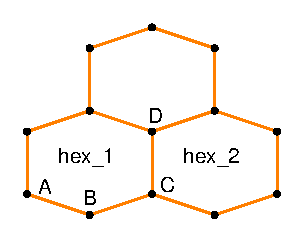
\includegraphics[width=4cm]{malha-hex.eps}} }
\medskip

Consider the mesh {\codett hex\_msh} shown above, made of three hexagons.
Pick one of them, at random :

\verbatim
   CellIterator it1 = hex_msh.iter_over ( tag::cells_of_dim, 2 );
   it1.reset();
   Cell hex_1 = *it1;
\endverbatim

Now choose a random segment on the boundary of {\codett hex\_1} :

\verbatim
   CellIterator it2 = hex_1.boundary().iter_over ( tag::segments );
   it2.reset();
   Cell AB = *it2;
\endverbatim

Take its tip :

\verbatim
   Cell B = AB.tip();
\endverbatim

Suppose now we want the next segment, within the boundary of {\codett hex\_1} :

\verbatim
   Cell BC = hex_1.boundary().cell_in_front_of ( B );
\endverbatim

And now we may continue by taking the tip of {\codett BC} and then the segment
following it$\;$:

\verbatim
   Cell C = BC.tip();
   Cell CD = hex_1.boundary().cell_in_front_of ( C );
\endverbatim

\noindent an so forth (this is how iterators over vertices and segments of
one-dimensional meshes, described in paragraph \numb section 8.\numb parag 6,
are implemented internally).

Within the mesh {\codett hex\_msh}, we can navigate towards a neighbour hexagon :

\verbatim
   Cell hex_2 = hex_msh.cell_in_front_of ( CD );
\endverbatim

Since we have picked {\codett hex\_1} at random within {\codett hex\_msh},
as well as {\codett AB} within the boundary of {\codett hex\_1},
there is no guarantee that we actually are in the configuration shown in the
picture above.
That is, {\codett CD} may be on the boundary of {\codett hex\_msh};
there may be no neighbour hexagon {\codett hex\_2}.
If that is the case, the code above will produce an execution error.
See paragraph \numb section 8.\numb parag 9 for a way to check whether there is actually
a neighbour cell and thus avoid errors at execution time.

Note that faces point outwards.
For instance, {\codett CD} belongs to the boundary of {\codett hex\_1} and points
outwards, towards {\codett hex\_2}.
Thus, {\codett hex\_msh.cell\_in\_front\_of(CD)} produces {\codett hex\_2}.
On the other hand, {\codett hex\_msh.cell\_behind(CD)} is {\codett hex\_1}.

Note also that {\codett CD} does not belong to the boundary of {\codett hex\_2}.
If we take {\codett hex\_2.boundary() .cell\_in\_front\_of(D)} we will obtain not
{\codett CD} but its reverse, a distinct cell which we may call {\codett DC}.
We have that {\codett hex\_msh.cell\_in\_front\_of(DC)} is {\codett hex\_1} and
{\codett hex\_msh.cell\_behind(DC)} is {\codett hex\_2}.


\paragraph{\numb section 8.\numb parag 9. Navigating at the boundary of a mesh}

Consider the example in paragraph \numb section 8.\numb parag 8.
Suppose you try to get a neighbour hexagon which does not exist :

\verbatim
   Cell no_such_hex = hex_msh.cell_in_front_of ( AB );
\endverbatim

In {\codett DEBUG} mode, you will get an {\codett assertion error}.
In {\codett NDEBUG} mode, the behaviour is undefined
(often, a {\codett segmentation fault} will arise).
The {\codett DEBUG} mode is explained at the beginning of paragraph \numb section
9.\numb parag 12.

You may check the existence of the neighbour cell by using a
{\codett tag::may\_not\_exist} and then the cell's method {\codett exists} :

\verbatim
   Cell possible_hex = hex_msh.cell_in_front_of ( AB, tag::may_not_exist );
   if ( possible_hex.exists() ) do_something_to ( possible_hex );
   else cout << "no neighbour !" << endl;
\endverbatim

\noindent thus avoiding errors at execution time.

Paragraph \numb section 8.\numb parag 10 gives a complete list of operations which return
an existing cell or build a new one.


\paragraph{\numb section 8.\numb parag 10. Declaring cells and meshes}

As explained in paragraph \numb section 9.\numb parag 3, the {\codett Cell} class
is just a thin wrapper around a {\codett Cell::Core}, and similarly for {\codett Mesh}es.

Statements below build a new wrapper for an existing cell or mesh.
No new cell or mesh is created :

\verbatim
   Cell A = B;  // B is a Cell
   Cell C = *it;  // 'it' is a CellIterator
   Mesh msh_copy = msh;  // msh is a Mesh
   Mesh bd = cll.boundary();  // cll is a Cell of dimension at least 2
\endverbatim

Statements below search for an existing cell.
If the respective cell exists, (a new wrapper for) it is returned.
Otherwise, an {\codett assertion error} will occur in {\codett DEBUG} mode;
in {\codett NDEBUG} mode, the behaviour is undefined (often, a {\codett segmentation fault}
will arise).
The {\codett DEBUG} mode is explained at the beginning of paragraph \numb section
9.\numb parag 12.

\verbatim
   Cell A_rev = A.reverse ( tag::surely_exists );  //  A is a Cell
   // or, equivalently :
   Cell A_rev ( tag::reverse_of, A, tag::surely_exists );

   Cell tri1 = msh.cell_behind ( CD );  //  CD is a Cell, a face within msh
   Cell tri2 = msh.cell_in_front_of ( CD );
   // or, equivalently :
   Cell tri1 ( tag::behind_face, CD, tag::within_mesh, msh );
   Cell tri2 ( tag::in_front_of_face, CD, tag::within_mesh, msh );
   // or, equivalently :
   Cell tri1 = msh.cell_behind ( CD, tag::surely_exists );
   Cell tri2 = msh.cell_in_front_of ( CD, tag::surely_exists );
   // or, equivalently :
   Cell tri1 ( tag::behind_face, CD, tag::within_mesh, msh, tag::surely_exists );
   Cell tri2 ( tag::in_front_of_face, CD,
               tag::within_mesh, msh, tag::surely_exists );
\endverbatim

Note that reverse meshes exist always (negative meshes are temporary objects built
on-the-fly).

\verbatim
   Mesh rev_msh = msh.reverse();  // msh is a Mesh
\endverbatim

Statements below search for an existing cell.
If the respective cell exists, (a new wrapper for) it is returned.
Otherwise, a non-existent cell is returned
(an empty wrapper); the user has the possibility of inquiring the existence
of the returned cell using its method {\codett exists}, as illustrated in paragraph
\numb section 8.\numb parag 9.

\verbatim
   Cell A_rev = A.reverse ( tag::may_not_exist );  //  A is a Cell
   // or, equivalently :
   Cell A_rev ( tag::reverse_of, A, tag::may_not_exist );
   
   Cell tri1 = msh.cell_behind ( CD, tag::may_not_exist );
   //  CD is a Cell, a face within msh
   Cell tri2 = msh.cell_in_front_of ( CD, tag::may_not_exist );
   // or, equivalently :
   Cell tri1 ( tag::behind_face, CD, tag::within_mesh, msh, tag::may_not_exist );
   Cell tri2
      ( tag::in_front_of_face, CD, tag::within_mesh, msh, tag::may_not_exist );
\endverbatim

Statements below return a previously built cell, if it exists.
If that object does not exist, it is built on-the-fly.

\verbatim
   Cell A_rev = A.reverse();  // A is some Cell
   // or, equivalentely :
   Cell A_rev ( tag::reverse_of, A );
   // or, equivalentely :
   Cell A_rev = A.reverse ( tag::build_if_not_exists );
   // or, equivalentely :
   Cell A_rev ( tag::reverse_of, A, tag::build_if_not_exists );
\endverbatim

Statements below return a wrapper for a brand new cell or mesh :

\verbatim
   Cell A ( tag::vertex );
   Mesh AB ( tag::segment, A.reverse(), B, tag::divided_in, 15 );
   // B is another vertex Cell
   Mesh ABC ( tag::triangle, AB, BC, CA );
   //  BC and CA are segment Meshes, each having 15 segments Cells
   // ... and many other shapes ...
\endverbatim

Paragraph \numb section 9.\numb parag 6 explains similar operations on {\codett Cell::Core}s.
